\documentclass[letterpaper,10pt]{article}

\usepackage{titling}
\usepackage{listings}
\usepackage{url}
\usepackage{setspace}
\usepackage{subfig}
\usepackage{sectsty}
\usepackage{pdfpages}
\usepackage{colortbl}
\usepackage{multirow}
\usepackage{relsize}
\usepackage{amsmath}
\usepackage{fancyvrb}
\usepackage{amsmath,amssymb,amsthm,graphicx,xspace}
\usepackage[titlenotnumbered,noend,noline]{algorithm2e}
\usepackage[compact]{titlesec}
\usepackage{paratype} 
\usepackage[T1]{fontenc}
\usepackage{tikz}
\usetikzlibrary{arrows,automata,shapes,trees,matrix,chains,scopes,positioning,calc}
\tikzstyle{block} = [rectangle, draw, fill=blue!20, 
    text width=2.5em, text centered, rounded corners, minimum height=2em]
\tikzstyle{bw} = [rectangle, draw, fill=blue!20, 
    text width=4em, text centered, rounded corners, minimum height=2em]

\definecolor{namerow}{cmyk}{.40,.40,.40,.40}
\definecolor{namecol}{cmyk}{.40,.40,.40,.40}

\let\LaTeXtitle\title
\renewcommand{\title}[1]{\LaTeXtitle{\textsf{#1}}}


\newcommand{\handout}[5]{
  \noindent
  \begin{center}
  \framebox{
    \vbox{
      \hbox to 5.78in { {\bf ECE254: Operating Systems and Systems Programming } \hfill #2 }
      \vspace{4mm}
      \hbox to 5.78in { {\Large \hfill #4  \hfill} }
      \vspace{2mm}
      \hbox to 5.78in { {\em #3 \hfill} }
    }
  }
  \end{center}
  \vspace*{4mm}
}

\newcommand{\lecture}[3]{\handout{#1}{#2}{#3}{Lecture #1}}
\newcommand{\tuple}[1]{\ensuremath{\left\langle #1 \right\rangle}\xspace}

\addtolength{\oddsidemargin}{-1.000in}
\addtolength{\evensidemargin}{-0.500in}
\addtolength{\textwidth}{2.0in}
\addtolength{\topmargin}{-1.000in}
\addtolength{\textheight}{1.75in}
\addtolength{\parskip}{\baselineskip}
\setlength{\parindent}{0in}
\renewcommand{\baselinestretch}{1.5}
\newcommand{\term}{Spring 2015}

\singlespace


\begin{document}

\lecture{ 18 --- Concurrency \& Synchronization in UNIX }{\term}{Jeff Zarnett}

\section*{Concurrency with pthreads}

Earlier we saw pthreads and how we can use them to have multithreaded programs. There are, accordingly, pthread routines for working with mutual exclusion (mutexes).

The first function of note is \texttt{pthread\_mutex\_init} which is used to create a new mutex variable and returns it, with type \texttt{pthread\_mutex\_t}. It takes an optional parameter, the attributes (the details of which are not important at the moment, but relate mostly to priorities). We can initialize it using null, but there is also a syntactic shortcut to do static initialization if you do not want to set attributes~\cite{pthreads}: \\ \texttt{pthread\_mutex\_t mymutex = PTHREAD\_MUTEX\_INITIALIZER;} 

When created, by default, the mutex is unlocked. There are three methods related to using the mutex; two to lock it and one to unlock it, all of which take as a parameter the mutex to (un)lock. The unlock method, \texttt{pthread\_mutex\_unlock} is self-explanatory. The two kinds of lock are \texttt{pthread\_mutex\_lock}, which is blocking, and \texttt{pthread\_mutex\_trylock}, which is nonblocking. As expected, attempting to unlock a mutex that is not currently locked is an error, but it is also an error if one thread attempts to unlock a mutex owned by another thread~\cite{pthreads}.

To destroy a mutex, there is a method \texttt{pthread\_mutex\_destroy}. As expected, it cleans up a mutex and should be used when finished with it. If attributes were created with \texttt{pthread\_mutexattr\_init} they should be destroyed with \texttt{pthread\_mutexattr\_destroy}.

An attempt to destroy the mutex may fail if the mutex is currently locked. The specification says that destroying an unlocked mutex is okay, but attempting to destroy a locked one results in undefined behaviour. Undefined behaviour is, in the words of the internet, the worst thing ever: it means code might work some of the time or on some systems, but not others, or could work fine for a while and then break suddenly later when something else is changed\footnote{Sadly, the specifications for C and POSIX and many other things are riddled with these ``undefined behaviour'' situations and it causes programmers everywhere a great deal of stress and difficulty. Another example: reading from an uninitialized variable in C produces undefined behaviour too.}.

\subsection*{Condition Variables}
Condition variables are another way to achieve synchronization. Rather than designating critical areas and enforcing rules about how many threads may be in the critical area, a condition variable allows synchronization based on the value of the data. Instead of locking a mutex, checking a variable, and then unlocking the mutex, we could achieve the same goal without constantly polling. We can think of condition variables as ``events'' that occur (like interrupts from hardware when there is new data to read rather than polling to check periodically or constantly).

An event is similar to, but slightly different from, a counting semaphore. We have the option, when an event occurs, to signal either one thread waiting for that event to occur, or to broadcast (signal) to all threads waiting for the event~\cite{mte241}. It should be noted that if a thread signals a condition variable that an event has occurred, but no thread is waiting for that event, the event is ``lost''. 

Condition variables are also supported in pthreads (as you probably guessed from its appearance in this section). To create a \texttt{pthread\_cond\_t} (condition variable type), the function is \texttt{pthread\_cond\_init} and to destroy them, \texttt{pthread\_cond\_destroy}. As before, we can initialize them with attributes, and there are functions to create and destroy the attribute structures, too. 

Condition variables are a building block and must be paired with a mutex. To wait on a condition variable, the function \texttt{pthread\_cond\_wait} takes two parameters: the condition variable and the mutex. This routine should be called only while the mutex is locked. It will automatically release the mutex while it waits for the condition; when the condition is true then the mutex will be automatically locked again so the thread may proceed. The programmer then unlocks the mutex when the thread is finished with it~\cite{pthreads}. Obviously, failing to lock and unlock the mutex before and after using the condition variable, respectively, can result in problems.

In addition to the expected \texttt{pthread\_cond\_signal} function that signals a provided condition variable, there is also \texttt{pthread\_cond\_broadcast} that signals all threads waiting on that condition variable. Because an event that takes place when no thread is listening is simply lost, it is (almost always) a logical error to signal or broadcast on a condition variable before some thread is waiting on it.

\paragraph{Condition Variable Example.} Let us now examine a code example from~\cite{pthreads}:
{\scriptsize
\begin{verbatim}
#include <pthread.h>
#include <stdio.h>
#include <stdlib.h>

#define NUM_THREADS  3
#define TCOUNT 10
#define COUNT_LIMIT 12

int     count = 0;
pthread_mutex_t count_mutex;
pthread_cond_t count_threshold_cv;

void *inc_count(void *t) {
  int i;
  long my_id = (long)t;

  for (i=0; i < TCOUNT; i++) {
    pthread_mutex_lock(&count_mutex);
    count++;

    /* Check the value of count and signal waiting thread when condition is
    reached.  Note that this occurs while mutex is locked. */
    if (count == COUNT_LIMIT) {
      printf("inc_count(): thread %ld, count = %d  Threshold reached. ",
             my_id, count);
      pthread_cond_signal(&count_threshold_cv);
      printf("Just sent signal.\n");
      }
    printf("inc_count(): thread %ld, count = %d, unlocking mutex\n", 
       my_id, count);
    pthread_mutex_unlock(&count_mutex);

    /* Do some work so threads can alternate on mutex lock */
    sleep(1);
    }
  pthread_exit(NULL);
}

void *watch_count(void *t) {
  long my_id = (long)t;

  printf("Starting watch_count(): thread %ld\n", my_id);

  /* Lock mutex and wait for signal.  Note that the pthread_cond_wait routine
  will automatically and atomically unlock mutex while it waits. 
  Also, note that if COUNT_LIMIT is reached before this routine is run by
  the waiting thread, the loop will be skipped to prevent pthread_cond_wait
  from never returning. */
  pthread_mutex_lock(&count_mutex);
  
  while (count < COUNT_LIMIT) {
    printf("watch_count(): thread %ld Count= %d. Going into wait...\n", my_id,count);
    pthread_cond_wait(&count_threshold_cv, &count_mutex);
    printf("watch_count(): thread %ld Condition signal received. Count= %d\n", my_id,count);
    printf("watch_count(): thread %ld Updating the value of count...\n", my_id,count);
    count += 125;
    printf("watch_count(): thread %ld count now = %d.\n", my_id, count);
    }
  printf("watch_count(): thread %ld Unlocking mutex.\n", my_id);
  pthread_mutex_unlock(&count_mutex);
  pthread_exit(NULL);
}

int main(int argc, char *argv[]) {
  int i, rc; 
  long t1=1, t2=2, t3=3;
  pthread_t threads[3];
  pthread_attr_t attr;

  /* Initialize mutex and condition variable objects */
  pthread_mutex_init(&count_mutex, NULL);
  pthread_cond_init (&count_threshold_cv, NULL);

  /* For portability, explicitly create threads in a joinable state */
  pthread_attr_init(&attr);
  pthread_attr_setdetachstate(&attr, PTHREAD_CREATE_JOINABLE);
  pthread_create(&threads[0], &attr, watch_count, (void *)t1);
  pthread_create(&threads[1], &attr, inc_count, (void *)t2);
  pthread_create(&threads[2], &attr, inc_count, (void *)t3);

  /* Wait for all threads to complete */
  for (i = 0; i < NUM_THREADS; i++) {
    pthread_join(threads[i], NULL);
  }
  printf ("Main(): Waited and joined with %d threads. Final value of count = %d. Done.\n", 
          NUM_THREADS, count);

  /* Clean up and exit */
  pthread_attr_destroy(&attr);
  pthread_mutex_destroy(&count_mutex);
  pthread_cond_destroy(&count_threshold_cv);
  pthread_exit (NULL);

}
\end{verbatim}
}

\subsection*{Monitors}
A condition variable can be used to create a \textit{monitor}, a higher level synchronization construct. Just as in object-oriented programming we package up data and functions inside a class to make errors less likely and to improve the design, when we use a monitor we are packaging up the shared data and operations on that data to avoid problems of synchronization and concurrency.

The objective of the monitor is to make it so that programmers do not need to code the synchronization part directly, making it less likely a programmer makes an error.

\begin{center}
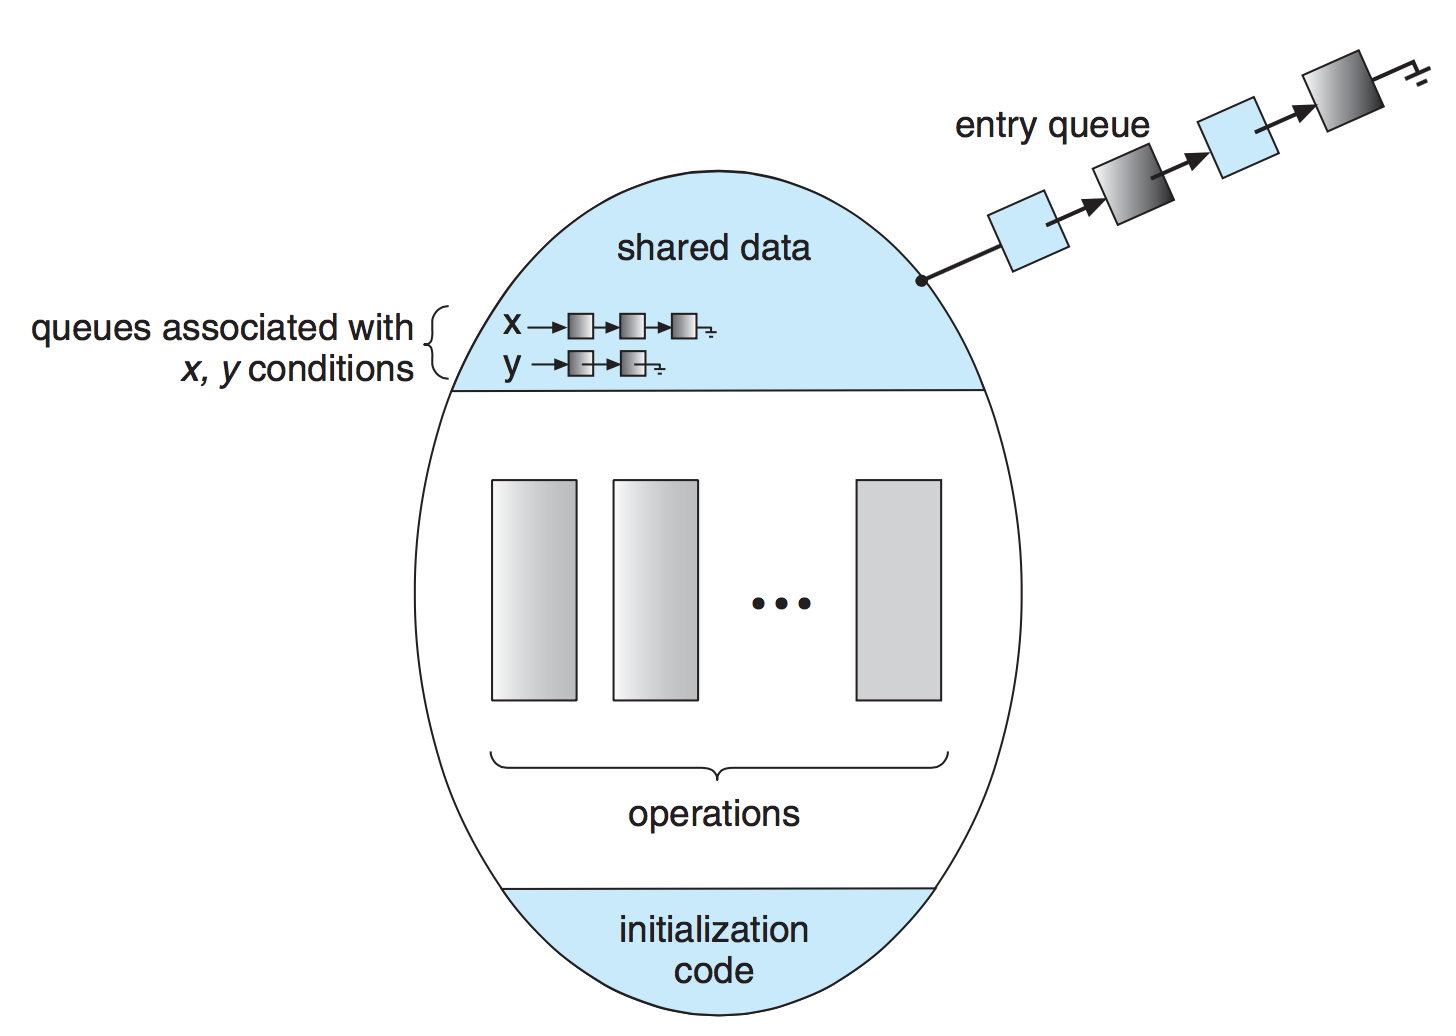
\includegraphics[width=0.65\textwidth]{images/sync-monitor.png}\\
Conceptual view of a monitor~\cite{osc}.
\end{center}

Suppose there are processes $P$ and $Q$ and a condition variable $x$. If $P$ signals on $x$ when $Q$ is waiting, there are two things we can do: \textit{signal-and-wait}, where $P$ waits until $Q$ leaves the monitor (or another condition); or \textit{signal-and-continue} where $P$ continues and $Q$ waits for $P$ to leave the monitor or another condition. Signal-and-continue seems logical, in one sense: $P$ is already running, so why do the extra work to switch? On the other hand, by the time $P$ exits the monitor on its own, the condition $Q$ was waiting for might no longer be true. Some programming languages opt for a compromise: after signalling, $P$ must immediately leave the monitor~\cite{osc}.

The idea of monitors should be familiar to you if you have used Java synchronization constructs, notably the \texttt{synchronized} keyword. In Java we can declare a method to be \texttt{synchronized}, adding it after the access modifier keyword (public, private, etc) in the function definition, and then there is a lock created around that method. Only one thread can be inside that method at a time; if a second would like to call that method on the same instance, it will be placed in the entry set for the lock: a set of threads waiting for the lock to become available~\cite{osc}. 

\begin{verbatim}
public synchronized void doSomething() {
    // Synchronized area
}
\end{verbatim}


Note that in Java we can make a method \texttt{synchronized} or define a block as synchronized:

\begin{verbatim}
public void exampleMethod() {
    synchronized( object ) { // Lock must be acquired to enter this block
           // Critical section 
    } // Lock is automatically released.
}
\end{verbatim}

This sort of ``automatic'' locking and releasing is intended to simplify the process of writing multithreaded code and abstract away the details of mutual exclusion.

\section*{Concurrency Mechanisms in UNIX-Like Systems}

We have already mentioned the idea of pipes, shared memory, and signals as ways of having inter-process (or inter-thread) communication in UNIX. UNIX also has semaphores (not just in the pthreads). The semaphore in UNIX is a general semaphore, and maintains a few pieces of extra data~\cite{osi}:
\begin{itemize}
    \item The value of the semaphore.
    \item Process ID of the last process to operate it.
    \item Number of processes waiting on a value greater than the current value.
    \item Number of processes waiting for the value to be 0.
\end{itemize}

UNIX semaphores are technically created in sets of one or more. It is possible to manage semaphores en masse with a system call (\texttt{semctl}), which then performs the requested operation on all of the semaphores in the set. There is also a \texttt{sem\_op} system call that takes as an argument, a list of semaphore operations, each defined on one of the semaphores in the set. When \texttt{sem\_op} is used, the indicated operations are performed one at a time. The usage of \texttt{sem\_op} is as follows~\cite{osi}:
\begin{itemize}
    \item \texttt{sem\_op} positive: increment the value of the semaphore and wake up any processes waiting on that semaphore.
    \item \texttt{sem\_op} 0: if the semaphore value is currently 0, do nothing. Otherwise, block the process until the semaphore is 0, and increment the number of processes waiting for this to be 0.
    \item \texttt{sem\_op} negative and its absolute value less than or equal to the semaphore value: add \texttt{sem\_op} to the semaphore value, and if this makes the semaphore 0, wake up processes waiting for the semaphore to be 0.
    \item \texttt{sem\_op} negative and its absolute value greater than the semaphore value: block the process until the semaphore value is increased, and increment the number of processes waiting for the semaphore to be increased.
\end{itemize}

\subsection*{Linux Kernel Concurrency Mechanisms}

In addition to the standard UNIX concurrency mechanisms, Linux has concurrency mechanisms all its own, to provide concurrency in execution of kernel code. 

Atomic operations

Spinlocks

Semaphores

Barriers



\bibliographystyle{alpha}
\bibliography{254}


\end{document}